\section{REFERENCIAL TEÓRICO}
Nesta seção será apresentado os principais conceitos utilizados neste trabalho, como a modelagem do motor de corrente contínua utilizada; Filtro de Kalman; Teórica de Controle para sistema de primeira ordem; Controlador FeedForward; Comunicação Bluetooth entre outras coisas.

\subsection{Modelagem Motor de Corrente Contínua}
% Colocar imagem
Motores geram potência mecânica, de forma que a velocidade de rotação $\omega$ é o sinal de saída e a tensão aplicada é o sinal de entrada. 

% figura retirada do livro texto da disciplina de modelagem.
% FAZER FIGURA PRÓPRIA
\begin{figure}[H]
    \centering
    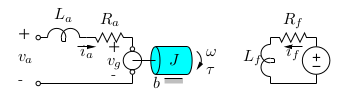
\includegraphics{imagens/ilustracoes/motor_cc_diagrama_modelo.png}
    \caption{Diagrama esquemático de um motor CC}
    \label{fig:modelo_motorcc}
\end{figure}

A figura \ref{fig:modelo_motorcc} apresenta o diagrama esquemático para um motor de corrente contínua (CC) controlado pela armadura, ou seja, o sinal de entrada é a tensão aplicada na armadura ($v_a$). Nesse diagrama a carga está sendo modelada por um momento de inércia $J$ e um atrito viscoso de coeficiente $b$.

\begin{align*}
    v_g &= K_{1}\phi\omega= K_{1}K_{2}i_{f}\omega = K_{m}\omega\\
    \tau &= K_{1} \phi i_{a}= K_{1} K_{2}i_{f} i_{a} = K_{m}i_{a}
\end{align*}

A constante $K_{m}$ é conhecida como a constante do motor. Devido a relação apresentada anterior, possível modelar o circuito equivalente do motor CC como na imagem \ref{fig:eq_eletrico_motorcc}.
% figura retirada do livro texto da disciplina de modelagem.
% FAZER FIGURA PRÓPRIA
\begin{figure}[H]
    \centering
    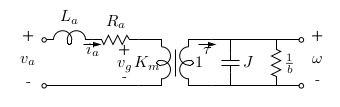
\includegraphics{imagens/ilustracoes/motor_cc_eq_eletrico.png}
    \caption{Equivalente elétrico de um motor CC}
    \label{fig:eq_eletrico_motorcc}
\end{figure}

Do circuito da figura \ref{fig:eq_eletrico_motorcc} extrai-se a seguinte função de transferência:

\begin{equation*}
    \frac{\Omega(s)}{V_a{s}} = \frac{K_m}{JL_{a}s^2 + \left(JR_a + BL_a \right)s + BR_a + K_{m}^2} \left[\frac{ rad.s^{-1}}{V}  \right]
\end{equation*}

Caso a impedância da armadura seja desprezada $(L_a \xrightarrow{} 0)$:

\begin{equation}
    \frac{\Omega(s)}{V_{a}(s)} = \frac{K_m}{JR_{a}s + BR_{a} + K_{m}^2} = \frac{K}{T_{m}s + 1} \left[\frac{ rad.s^{-1}}{V}  \right]
    \label{eq:motor_transf_func}
\end{equation}

Portando, caso a impedância da armadura seja desprezada, a função de transferência do motor que relacionada a velocidade angular com a tensão de entrada se comporta como um sistema de primeira ordem.

\subsection{Sistemas de Controle}

\begin{figure}[H]
    \centering
    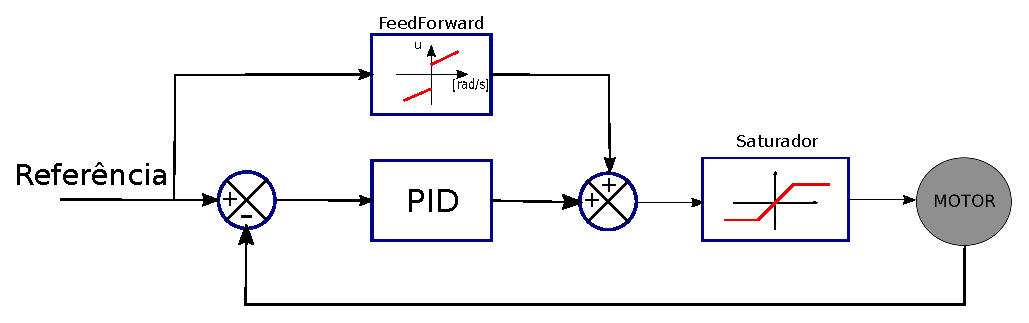
\includegraphics[width=\textwidth]{imagens/ilustracoes/sistema_de_controle_completo.eps}
    \caption{Diagrama de um sistema de controle \textit{FeedForward} + \textit{Backward}}
    \label{fig:diagrama_sistema_de_controle_feedforward_backward}
\end{figure}

\subsubsection{Controlador PID}

\subsubsection{Controlador FeedForward}

\subsubsection{Controlador FeedForward/Backward}

% Breve introdução à teoria de controle 
% modelagem utilizada para o trabalho atual, sistema motor/roda considerado
\subsection{Mínimos Quadrados}

\subsection{Filtro de Kalman}
% Introdução ao filtro de Kalman

Modelo do sistema:
\begin{equation}
\textbf{x}_k = F_x x_{k-1} + B_k u_k + w_k; w_k \sim N(0, Q_k)
\end{equation}

Modelo da medição:
\begin{equation}
z_k = H_k x_k + v_k; v_k \sim N(0, R_k)
\end{equation}

Predição:
\begin{align*}
    \check{x}_k &= F_k \hat{x}_{k-1} + B_k u_k\\
    \check{P}_k &= F_k \hat{P}_{k-1} F^T_k + Q_k
\end{align*}

Atualização:
\begin{align*}
    K_k &= \check{P}_k H^T \left( H_k \check{P}_k H^T_k + R_k\right)^{-1}\\
    \hat{x}_k &= \check{x}_k + K_k\left( z_k - H_k \check{x}_k \right)\\
    \hat{P}_k &= \left(I - KH_k \right)\check{P}_k
\end{align*}

% \subsubsection{Filtro de \textit{Kalman} para um sistema de primeira ordem}

\subsection{Bluetooth}
% Breve introdução à historia do bluetooth e utilidade
% destacar: custo energético, velocidade de operação, robustez a interferências

A  tecnologia \emph{Bluetooth}  suporta várias opções de topologia, incluindo conexões simples ponto a ponto. Operando na faixa de frequência industrial, científica e médica de $2,4$ GHz, a tecnologia \emph{Bluetooth} suporta várias opções de rádio.
    
O rádio \emph{Bluetooth} BR/EDR opera com baixo consumo de energia e também utiliza uma abordagem robusta de \textit{Adaptive Frequency Hopping}, transmitindo dados por $79$ canais. O \textit{Bluetooth} BR/EDR inclui várias opções de \textit{PHY} que suportam taxas de dados de $1$ Mb a $3$ Mb e suporta vários níveis de energia, de $1$mW a $100$ mW, além de várias opções de segurança.

% aprofundar mais? 

\subsection{\textit{Encoders} Rotativos}
% Referencias:
% https://www.roboticsbusinessreview.com/news/differences-between-encoder-resolution-accuracy-and-precision/

% FALAR SOBRE O FUNCIONAMENTO BASICO
% CITAR OS DIFERENTES TIPOS
% FALAR DO GRAY CODE


\subsection{FreeRTOS}
% É um sistema operacional de tempo real.
% introduzir o que um RTOS, e introduzir o FreeRTOS
O \emph{FreeRTOS} é um sistema operacional de tempo real para microcontroladores, e é o utilizado no microcontrolador usado neste trabalho. Ele é desenvolvido por diversas empresas e é um dos mais populares e usados no mercado. Com ele é possível gerenciar os recursos do microcontrolador, como lançar vários processos em mais de um núcleo, dentre outras coisas, assim como um sistema operacional convencional, porém mais leve, pois possui menos funcionalidades. O \emph{FreeRTOS} é distribuído gratuitamente sobre a licença \textit{MIT}.

% FALTA COMPLEMENTAR
